\section{Network Debugger}
\subsection{Overview}

The user of the network debugger provides a model of the network and a
set of experiments. For each experiment, the network debugger assesses
whether the experiment is consistent with the model, explaining why
(with a queryable proof) or why not (with queryable minimal fixes).

\subsection{Demonstration}

For purpose of demonstration, we will use the small network shown in Figure~\ref{figure:network}.
The user code which specifies this network model is shown in Listing~\ref{listing:network-model-def}.

The set of experiments in Listing~\ref{listing:experiments} tests our
model. In order to test our system, we purposefully introduced some
inconsistencies in our model with respect to the experiments:
\begin{itemize}
\item {\small\tt reaction r1} has its reactants and products swapped.
\item {\small\tt reaction r2} has no enzymes catalyzing it.
\item {\small\tt reaction r4} shouldn't actually be part of our model.
\end{itemize}

\begin{figure}[htb]
\centering
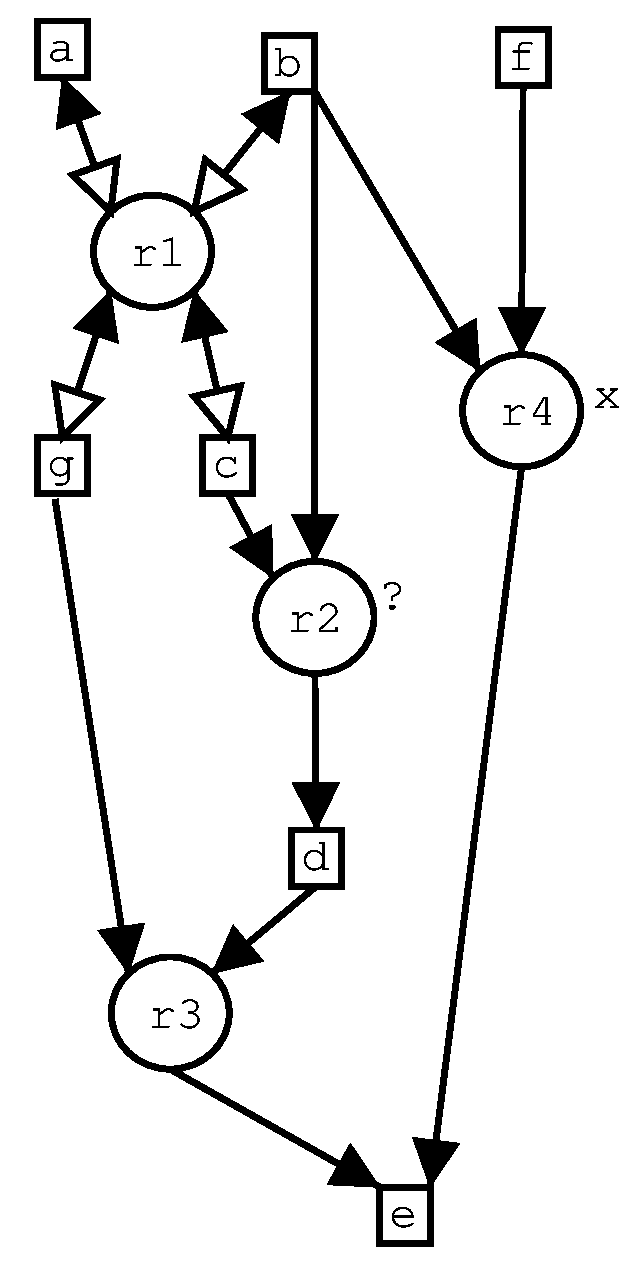
\epsfig{file=demo.eps, height=3in, width=1.5in}
\caption{\label{figure:network} Example Metabolic Network}
\end{figure}

\begin{lstlisting}[label={listing:network-model-def},caption={Network Model}]
(network-debugger demo 
  :debugging t 
  :abducting t 
  :rules :extended-reactions)

(reaction r1 
  :reactants (c g) 
  :products (a b) 
  :enzymes (e1))

(reaction r2 
  :reactants (b c) 
  :products (d))

(reaction r3 
  :reactants (d g) 
  :products (e) 
  :enzymes (e3))

(reaction r4 
  :reactants (b f) 
  :products (e) 
  :enzymes (e4))

(enzyme e1 g1)
(enzyme e3 g3 g3p)
(enzyme e4 g4)
\end{lstlisting}

\begin{lstlisting}[label={listing:experiments},caption={Experiments}]
(experiment 
 positive 
 (a b d) 
 :growth? t 
 :essential-compounds (a e))

(experiment 
 negative 
 (a) 
 :growth? nil 
 :essential-compounds (a e))

(experiment 
 false-positive 
 (a b f) 
 :growth? nil 
 :essential-compounds (a e) 
 :knock-outs (g1))

(experiment
 false-negative
 (a b)
 :growth? t
 :essential-compounds (a e))
\end{lstlisting}

We immediately get the following feedback when loading the set of
experiments:
\begin{itemize}
\item Experiments {\small\tt positive} and {\small\tt negative} are consistent with the model.
\item Experiment {\small\tt false-positive} is not consistent with the model. Needs:
\begin{itemize}
\item {\small\tt ( (NOT (GENE-ON G4)) )}
\end{itemize}
\item Experiment {\small\tt false-negative} is not consistent with the model. Needs:
\begin{itemize}
\item {\small\tt ( (NUTRIENT E) )}
\item {\small\tt ( (NUTRIENT D) )}
\item {\small\tt ( (REACTION-ENABLED R2) )}
\item {\small\tt ( (NUTRIENT F) )}
\end{itemize}
\end{itemize}

Notice that the network debugger suggested enabling {\small\tt
reaction r2} and disabling {\small\tt reaction r4} to fix our model.

Once an experiment is consistent with the model, the network debugger
can explain why by providing a proof and allowing the user to query
this proof. For example, after loading the experiment {\small\tt
positive}, the user can type {\small\tt (explain
'experiment-consistent)} to get a proof in the syle of
Suppes~\cite{suppes57}. The user can query the facts that play a role
in the proof using {\small\tt all-antecedents}. For example,
{\small\tt (all-antecedents 'experiment-consistent '((reaction-enabled
?r) (reaction-reversible ?r)))} returns {\small\tt ((REACTION-ENABLED
R3) (REACTION-ENABLED R1) (REACTION-REVERSIBLE R1))}. As a shortcut,
it is possible to list reactions that had to explicitly be assumed
reversible for the proof: {\small\tt (explicit-reversibility)} returns
{\small\tt (R1)}. Similarly, {\small\tt (explicit-gene-expression)}
returns which genes had to explicitly be assumed on for the proof.

\subsection{Specification}
\label{sec:spec}

We describe the user language to define the network model and experiments.

The network model consists of definitions of pathways, reactions, and enzymes.

An enzyme is defined by {\small\tt (enzyme <name> . <list of genes
(conjunctive)>}. The list of genes may contain {\small\tt :UNKNOWN} to
indicate that the enzyme has some unknown gene contributing to its
formation.

A pathway or reaction is defined by
{\small\tt (pathway/reaction <name> ...)} where {\small\tt ...} can contain any of the following keys:
\begin{description}
\item[:reactants] <list of reactants>
\item[:products] <list of products>
\item[:reversible?] <t / nil / :UNKNOWN> (By default, :UNKNOWN for reactions and nil for pathways.)
\item[:enzymes] <list of enzymes (disjunctive for reactions, unspecified logic for pathways)>
Note that
\begin{itemize}
\item nil for a reaction means that NO enzymes catalyze it, i.e. the reaction will never be fired but might play a role in abduction.
\item :SPONTANEOUS, instead of a list, means that no enzymes are needed.
\item (:UNKNOWN) means that some unknown enzyme is needed. :UNKNOWN can be part of any enzyme list.
\end{itemize}
\item[:reactions] <list of all reactions in the pathway> (pathways only)
\item[:proper-products] <list of the actual end products of a pathway> (pathways only) (This list should be a subset of products, and is the same as products by default.)
\end{description}

An experiment is defined by {\small\tt (experiment <name>
<nutrient-list> :growth? <T or nil> :essential-compounds <list of
compounds that must be produecd in order to achieve growth
(conjunctive)> ...)} where {\small\tt ...} can contain any of the
following:
\begin{description}
\item[knock-outs] <list of genes asserted to be off>
\item[knock-ins] <list of genes asserted to be on>
\item[toxins] <list of compounds that if produced cause no-growth experimental outcomes (disjunctive)>
\item[bootstrap-compounds] <list of compounds that are asserted to exist, but not nutrients>
\end{description}

\subsection{Implementation}

We implemented the network debugger on top of a logic-based truth maintenance system (LTMS)~\cite{bps93}.
Figure~\ref{figure:system} gives an overview of the system.

\begin{figure}[htb]
\centering
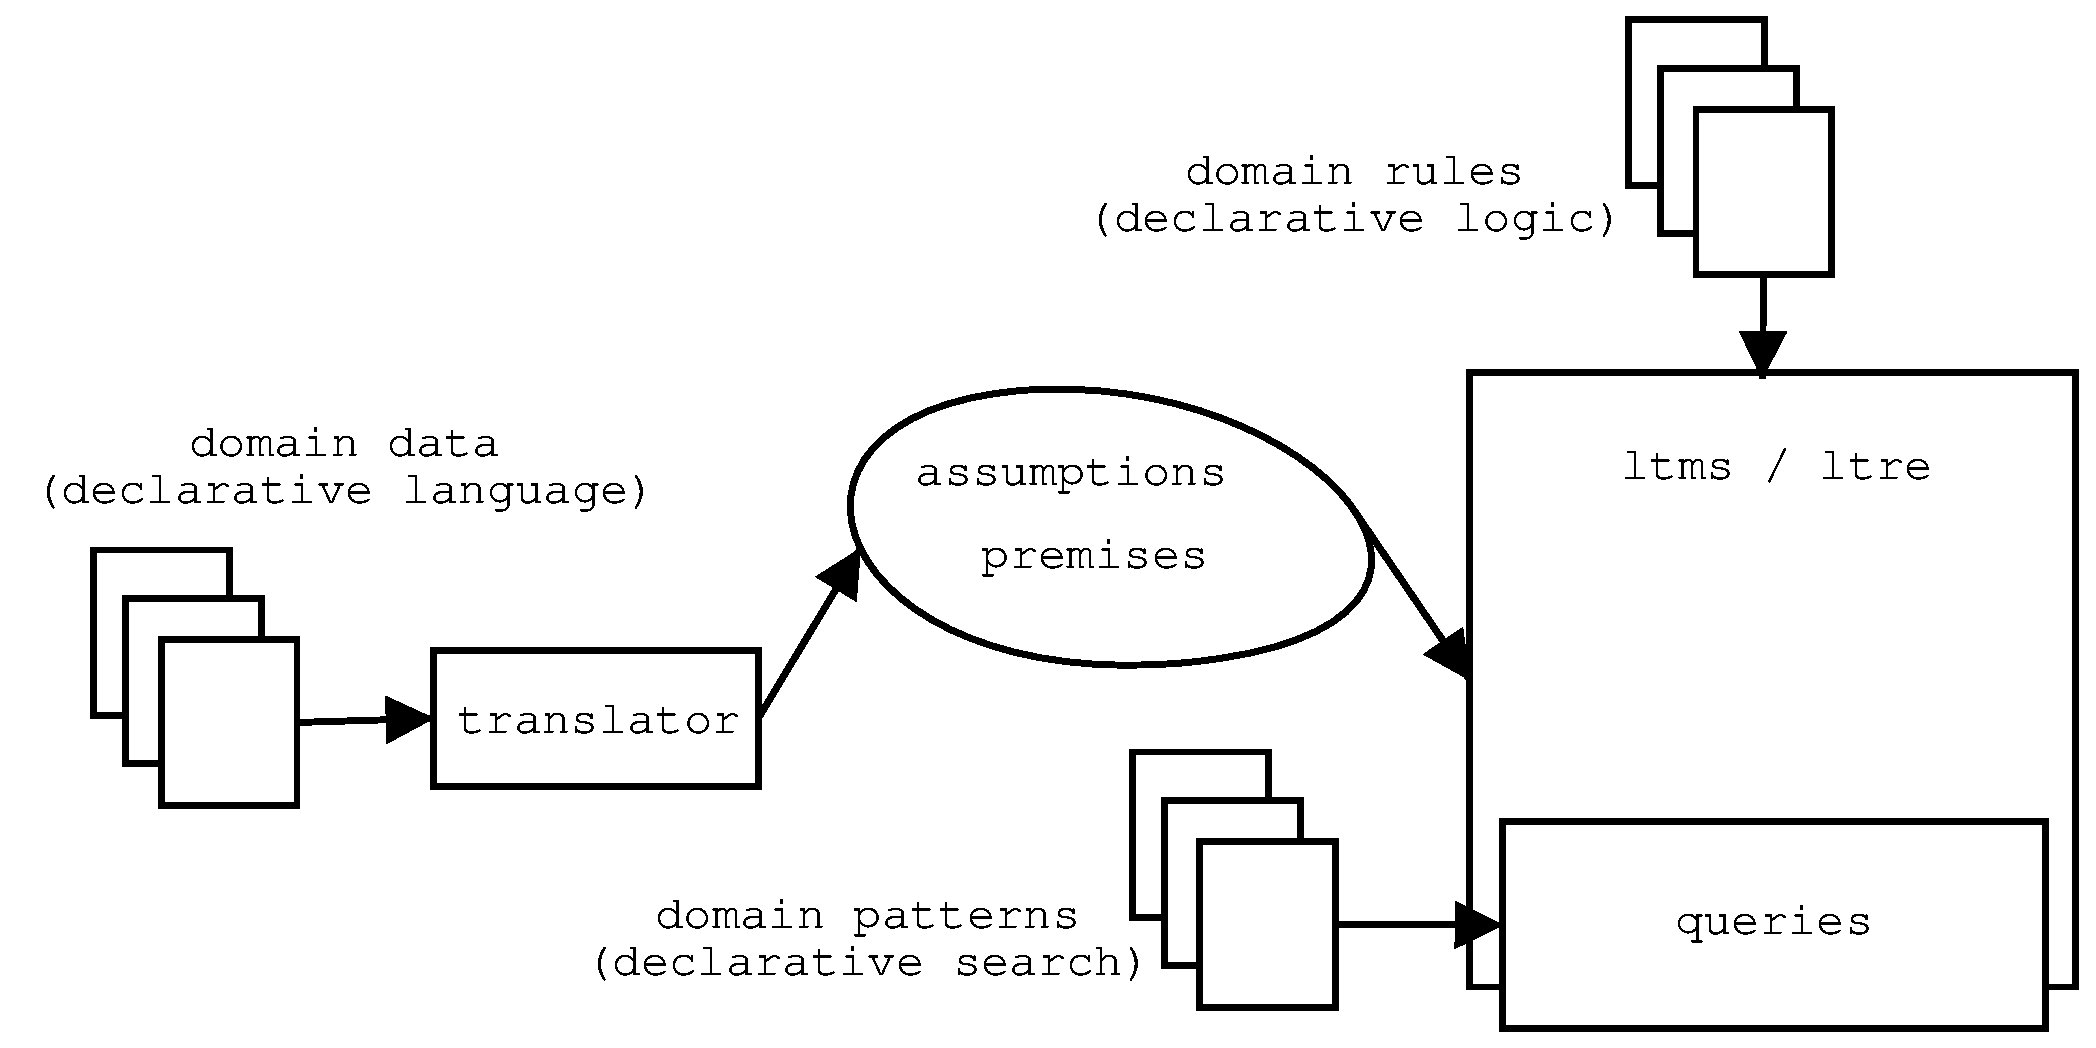
\epsfig{file=system.eps, height=2in, width=3in}
\caption{\label{figure:system} Overview of the Network Debugger System}
\end{figure}

Crucially, all our domain-specific knowledge is specified
declaratively. The domain data is given by the user, in the
domain-specific language outlined in~\ref{sec:spec}. The domain rules
are specified using the rule system of the LTMS engine. Finally, we
augmented the the query facility of the LTMS. The query facility is
still general. We apply it to our domain by restricting the queries
with patterns.

\subsubsection{Domain Data}

Using a straightforward set of macros, we translate the domain data
into assumptions and premises of our LTMS. For example, the macros for
{\small\tt enzyme} and {\small\tt experiment} are shown in
Listing~\ref{listing:enzyme-macro} and
Listing~\ref{listing:experiment-macro}. The network open / closed
distinction is explained in~\ref{sec:domain-rules}.

\begin{lstlisting}[label={listing:enzyme-macro},caption={Enzyme Macro}]
(defmacro enzyme (name &rest genes)
  `(ensure-network-open enzyme
    (assert! '(enzyme ,name ,@genes)
	     :NETWORK)
    (debugging-nd
     "~%Adding enzyme ~A." ',name)))
\end{lstlisting}

\begin{lstlisting}[label={listing:experiment-macro},caption={Experiment Macro}]
(defmacro experiment (name 
		      nutrients
		      &key
		      growth?
		      (knock-outs nil)
		      (knock-ins nil)
		      (toxins nil)
		      (bootstrap-compounds nil)
		      essential-compounds)
  `(ensure-network-closed 
    experiment
    (assert! '(experiment 
	       ,name ,growth? 
	       ,nutrients ,essential-compounds
	       ,bootstrap-compounds ,toxins
	       ,knock-ins ,knock-outs)
	     :EXPERIMENTS)
    (debugging-or-logging-nd
     "~%Adding experiment ~A" ',name)
    (run-rules-logging)
    (investigate-experiment ',name)))
\end{lstlisting}

\subsubsection{Domain Rules}
\label{sec:domain-rules}

The domain rules describe how to derive more facts from the premises
and assumptions. We can easily change the domain rules independently
of the rest of the system. For example, we have different sets of
rules, depending on whether the network debugger operates on pathways
or reactions.

Listing~\ref{listing:sample-rule} shows an excerpt of the domain
rules. It simply expresses the logic that if a reaction is enabled and
all the reactants are present, then the reaction is fired and all the
products are present.

\begin{lstlisting}[label={listing:sample-rule},caption={Excerpt of Domain Rules}]
(rule ((:INTERN (reaction 
                 ?reaction 
                 ?reactants ?products 
                 ?reversible? ?enzymes)))
  ...
  (assert! 
   `(:IMPLIES
     (:AND (reaction-enabled ,?reaction)
      ,@(list-of 'compound-present ?reactants))
    (:AND (reaction-fired ,?reaction)
      ,@(list-of 'compound-present ?products)))
   :REACTION-FIRED)
  ...
)
\end{lstlisting}

In addition to deriving positive facts, e.g. a certain compound is
present, we would like to be able to derive negative facts, e.g. a
certain compound is not present. However, in order to derive that a
compound is not present, we need to assume that the network is closed,
i.e. that no additional reactions are going to be
declared. Listing~\ref{listing:network-closed} shows the domain rule
that makes use of {\small\tt network-closed} premise.

\begin{lstlisting}[label={listing:network-closed},caption={Domain rule for deriving absence of compound}]
(rule ((:TRUE network-closed))
      (rule ((:INTERN (compound ?compound)))
(let* 
 ((product-facts 
   (fetch `(product ,?compound ?reaction)))
  (reactant-facts 
   (fetch `(reactant ,?compound ?reaction)))
  (reaction-fired-facts 
   (mapcar 
    #'(lambda (fact) 
      `(reaction-fired ,(caddr fact))) 
    product-facts))
  (reverse-reaction-fired-facts 
   (mapcar 
    #'(lambda (fact) 
      `(reverse-reaction-fired ,(caddr fact))) 
    reactant-facts)))
  (assert! 
   `(:IMPLIES 
     (:AND
      (:NOT (nutrient ,?compound))
      (:NOT 
       (:OR 
        ,@reaction-fired-facts 
        ,@reverse-reaction-fired-facts)))
      (:NOT (compound-present ,?compound)))
  :NETWORK-CLOSED))))
\end{lstlisting}

\subsubsection{Queries}

We extended the LTMS query facility with two procedures: {\small\tt
needs} and {\small\tt all-antecedents}. 

{\small\tt all-antecedents} is straightforward. It simply makes a list
of all facts that support a fact or recursively support any antecedent
of that fact.

{\small\tt needs} allows our system to perform abduction. It answers
the question: which unknown facts, if true, would be sufficient for a
given unknown fact to become true?

Both these procedures takes an optional list of patterns, which limits
the form of facts that can be returned.
